\subsection{Periodo di Progettazione di dettaglio e codifica}
\subsubsection{MQP01 - Indice di Gulpease}
\begin{table}[H]
    \rowcolors{2}{gray!25}{white}
    \rowcolors{2}{gray!25}{white}
        \renewcommand{\arraystretch}{1.5}
        \begin{tabular}{m{0.4\textwidth}<{\centering}  m{0.25\textwidth}<{\centering}  m{0.25\textwidth}<{\centering} }
            \rowcolor{darkblue}
            \textcolor{white}{\textbf{Documento}}& \textcolor{white}{\textbf{Valore}} & \textcolor{white}{\textbf{Esito}}\\ 

            \textit{NormeDiProgetto-v2.0.0} &
            65 &
            Superato \\

            \textit{PianoDiProgetto-v2.0.0} &
            73 &
            Superato \\

            \textit{PianoDiQualifica-v2.0.0} &
            66 &
            Superato \\

            \textit{AnalisiDeiRequisiti-v2.0.0} &
            88 &
            Superato \\
            
            \textit{Glossario-v2.0.0} &
            80 &
            Superato \\

            \textit{VerbaleEsterno-2022.03.03} &
            70 &
            Superato \\
            
            \textit{VerbaleEsterno-2022.04.08} &
            70 &
            Superato \\

            \textit{VerbaleEsterno-2022.04.28} &
            78&
            Superato \\

            \textit{VerbaleInterno-2022.02.23} &
            79&
            Superato \\
            \textit{VerbaleInterno-2022.02.28} &
            72&
            Superato \\
            \textit{VerbaleInterno-2022.03.07} &
            70&
            Superato \\
            \textit{VerbaleInterno-2022.03.14} &
            70&
            Superato \\
            \textit{VerbaleInterno-2022.04.04} &
            75&
            Superato \\
            \textit{VerbaleInterno-2022.04.11} &
            76&
            Superato \\
            \textit{VerbaleInterno-2022.04.25} &
            77&
            Superato \\
            \textit{VerbaleInterno-2022.05.09} &
            73&
            Superato \\
    \end{tabular}
    \caption{Progettazione di dettaglio e codifica: MQP01 - Indice di Gulpease}
\end{table}
\begin{figure}[H]
    \centering
    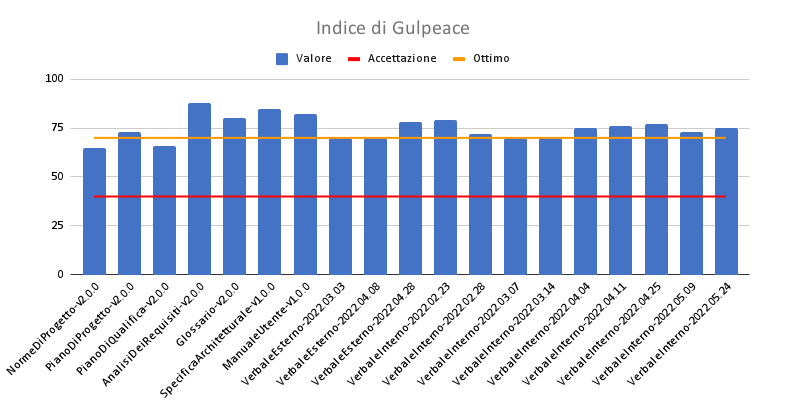
\includegraphics[scale=0.50]{Sezioni/images/pb_prodotto/Indice_di_Gulpeace.png}
    \caption{Progettazione di dettaglio e codifica: MPC02 - BCWS}
\end{figure}
\subsubsection{MQP02 - Profondità di una gerarchia}
\begin{figure}[H]
    \centering
    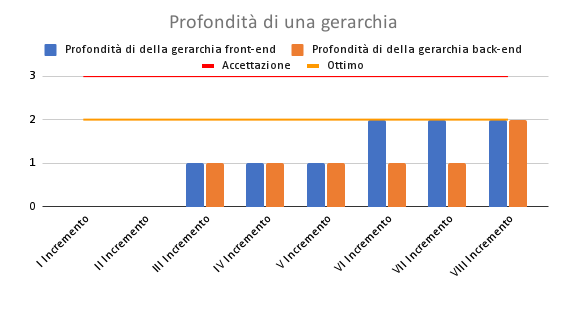
\includegraphics[scale=0.50]{Sezioni/images/pb_prodotto/Profondita_di_una_gerarchia.png}
    \caption{Progettazione di dettaglio e codifica: MQP02 - Profondità di una gerarchia}
\end{figure}
\subsubsection{MQP03 - Numero parametri per metodo}
\begin{figure}[H]
    \centering
    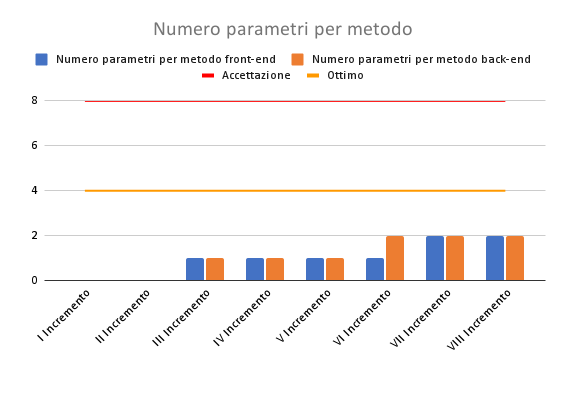
\includegraphics[scale=0.50]{Sezioni/images/pb_prodotto/Numero_parametri_per_metodo.png}
    \caption{Progettazione di dettaglio e codifica: MQP03 - Numero parametri per metodo}
\end{figure}
\subsubsection{MQP04 - Code coverage}
\begin{figure}[H]
    \centering
    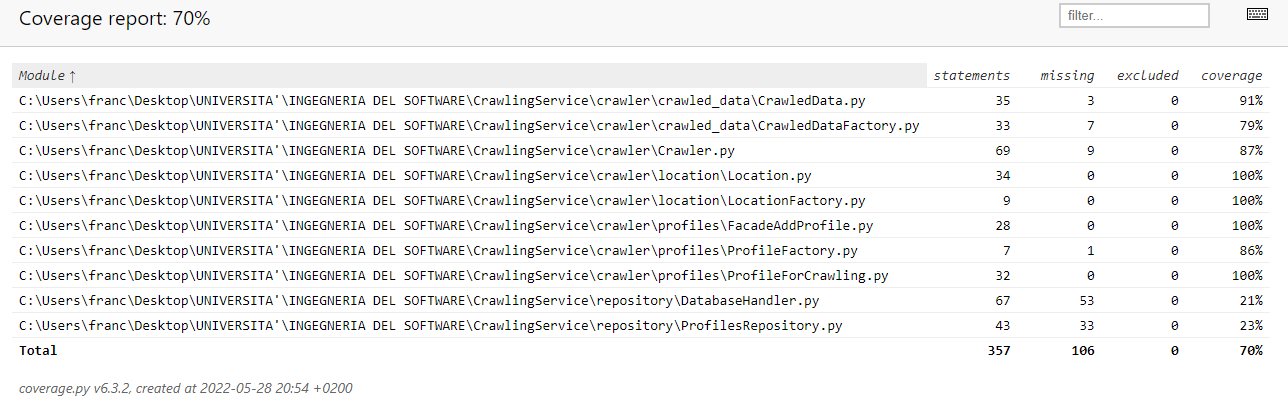
\includegraphics[scale=0.50]{Sezioni/images/pb_prodotto/coverage-CS.PNG}
    \caption{Progettazione di dettaglio e codifica: MQP04 - Code coverage - Crawling Service}
\end{figure}

\begin{figure}[H]
\centering
    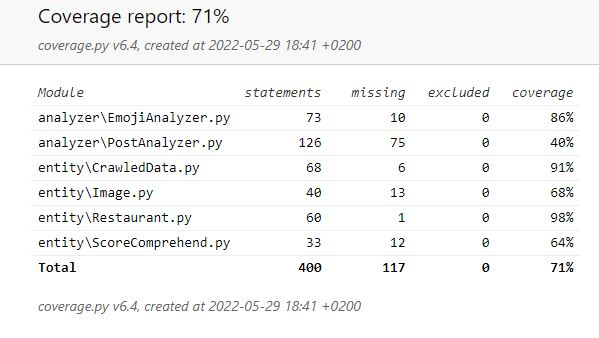
\includegraphics[scale=0.50]{Sezioni/images/pb_prodotto/coverage-RS.JPG}
    \caption{Progettazione di dettaglio e codifica: MQP04 - Code coverage - Ranking Service}
\end{figure}

\begin{figure}[H]
    \centering
    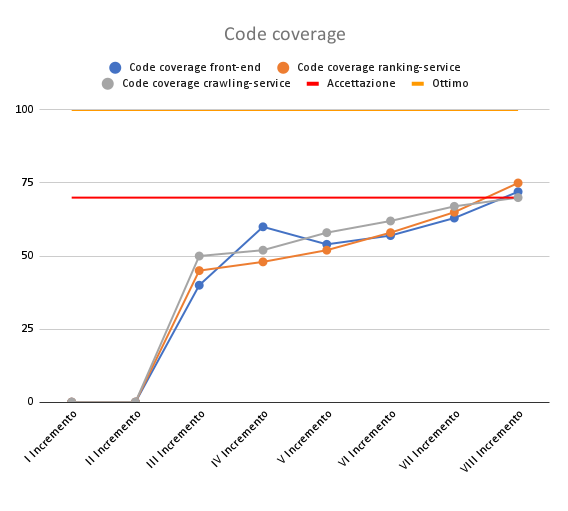
\includegraphics[scale=0.50]{Sezioni/images/pb_prodotto/Code_coverage.png}
    \caption{Progettazione di dettaglio e codifica: MQP04 - Code coverage}
\end{figure}
\subsubsection{MQP05 - Percentuale requisiti obbligatori soddisfatti}
\begin{figure}[H]
    \centering
    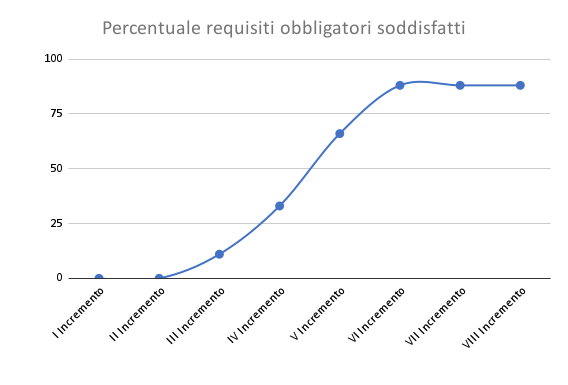
\includegraphics[scale=0.50]{Sezioni/images/pb_prodotto/Percentuale_requisiti_obbligatori_soddisfatti.png}
    \caption{Progettazione di dettaglio e codifica: MQP05 - Percentuale requisiti obbligatori soddisfatti}
\end{figure}
\subsubsection{MQP06 - Complessità ciclomatica}
\begin{figure}[H]
    \centering
    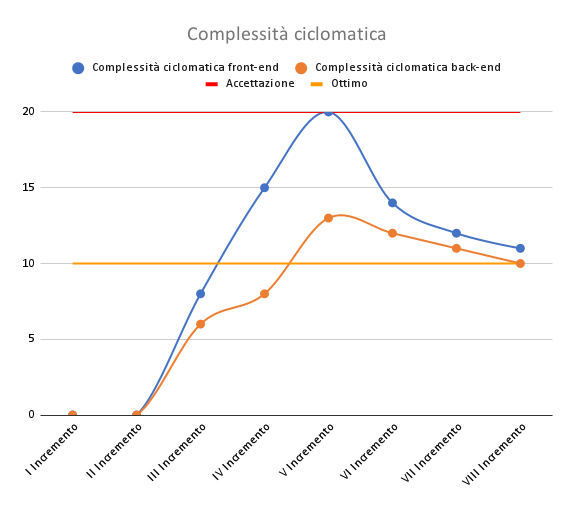
\includegraphics[scale=0.50]{Sezioni/images/pb_prodotto/Complessita_ciclomatica.png}
    \caption{Progettazione di dettaglio e codifica: MQP06 - Complessità ciclomatica}
\end{figure}
\subsubsection{MQP07 - Numero di bug}
\begin{figure}[H]
    \centering
    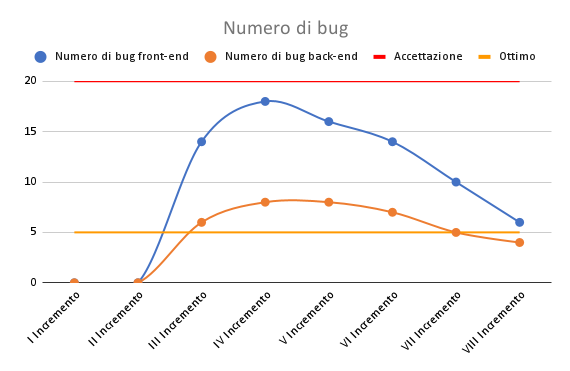
\includegraphics[scale=0.50]{Sezioni/images/pb_prodotto/Numero_di_bug.png}
    \caption{Progettazione di dettaglio e codifica: MQP07 - Numero di bug}
\end{figure}
\subsubsection{MQP08 - Numero di Code smell}
\begin{figure}[H]
    \centering
    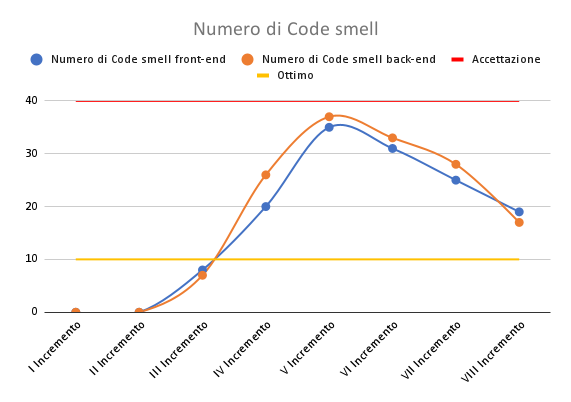
\includegraphics[scale=0.50]{Sezioni/images/pb_prodotto/Numero_di_Code_smell.png}
    \caption{Progettazione di dettaglio e codifica: MQP08 - Numero di Code smell}
\end{figure}
\subsubsection{MQP09 - Linee di Commento per Linee di Codice}
\begin{figure}[H]
    \centering
    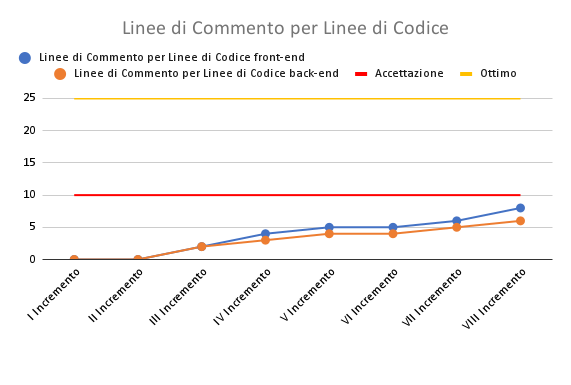
\includegraphics[scale=0.50]{Sezioni/images/pb_prodotto/Linee_di_Commento_per_Linee_di_Codice.png}
    \caption{Progettazione di dettaglio e codifica: MQP09 - Linee di Commento per Linee di Codice}
\end{figure}
\subsubsection{MQP10 - Branch Coverage}
\begin{figure}[H]
    \centering
    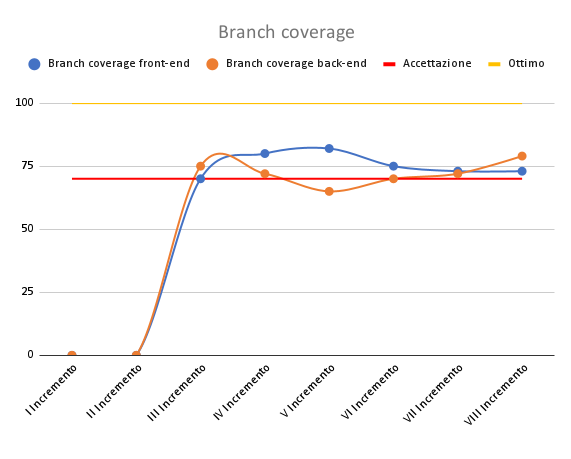
\includegraphics[scale=0.50]{Sezioni/images/pb_prodotto/Branch_coverage.png}
    \caption{Progettazione di dettaglio e codifica: MQP10 - Branch Coverage}
\end{figure}
\subsubsection{MQP11 - Successo di test}
\begin{figure}[H]
    \centering
    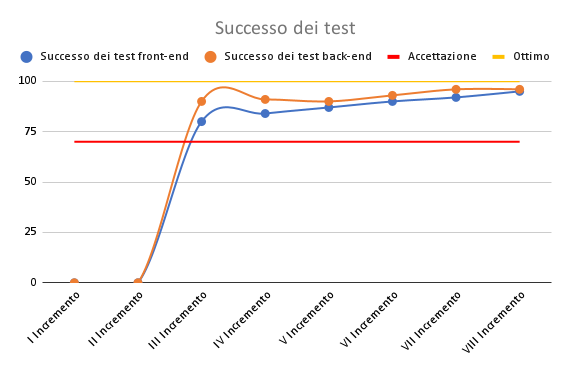
\includegraphics[scale=0.50]{Sezioni/images/pb_prodotto/Successo_dei_test.png}
    \caption{Progettazione di dettaglio e codifica: MQP11 - Successo di test}
\end{figure}
\subsubsection{MQP12 - Numero di vulnerabilità}
\begin{figure}[H]
    \centering
    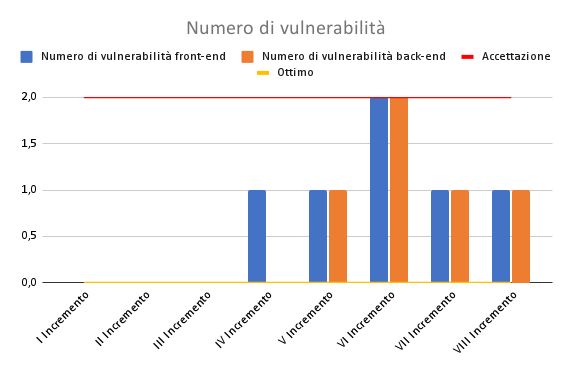
\includegraphics[scale=0.50]{Sezioni/images/pb_prodotto/Numero_di_vulnerabilita.png}
    \caption{Progettazione di dettaglio e codifica: MQP12 - Numero di vulnerabilità}
\end{figure}
